\documentclass[onecolumn]{article}
\usepackage{CJKutf8, graphicx}%导入CJKutf8包,并且激活中文、日文、韩文的uft8编码
\usepackage[utf8]{inputenc}
\usepackage{setspace}
\usepackage{indentfirst}
\usepackage{geometry}
\geometry{left=3.18cm,right=3.18cm,top=2.54cm,bottom=2.54cm}
\renewcommand{\baselinestretch}{1.5}

\title{短视频传输实验报告}
\author{计研173 \quad 陈雨兰 \quad 2017310787  \\ 计研173 \quad 蔡文静 \quad 2017210866}
\date{January 2018}

\begin{document}
	\begin{CJK*}{UTF8}{gbsn}
		
		\maketitle
\section{介绍}
		该项目实现了从客户端到服务器端的短视频的快速上传。我们在UDP协议传输数据的基础上加上了乱序恢复和丢包恢复,从而实现了短视频的快速准确的传输。
		
\section{项目设计与分析}
		\subsection{算法框架}
		为了应对UDP传输中的丢包和乱序的情况,我们采用前向纠错技术进行丢包恢复。
		该算法由发送方进行FEC编码引入冗余包,接收方进行FEC解码并恢复丢失的数据包。
		对于包乱序和包重复,我们采用QOS乱序恢复处理。
		%该QOS方案特点是在没有丢包的情况下,不引入任何系统延时,并且可以通过可控的丢包等待时延来适应不同的信道乱序程度。
		QOS需要在接收端进行FEC解码前进行,确保送FEC解码模块的数据包序号是正确的(不存在乱序,仅存在丢包)。
		图\ref{fig:frame}为算法的主要框架。
		
		\begin{figure}[h]
			\centering
			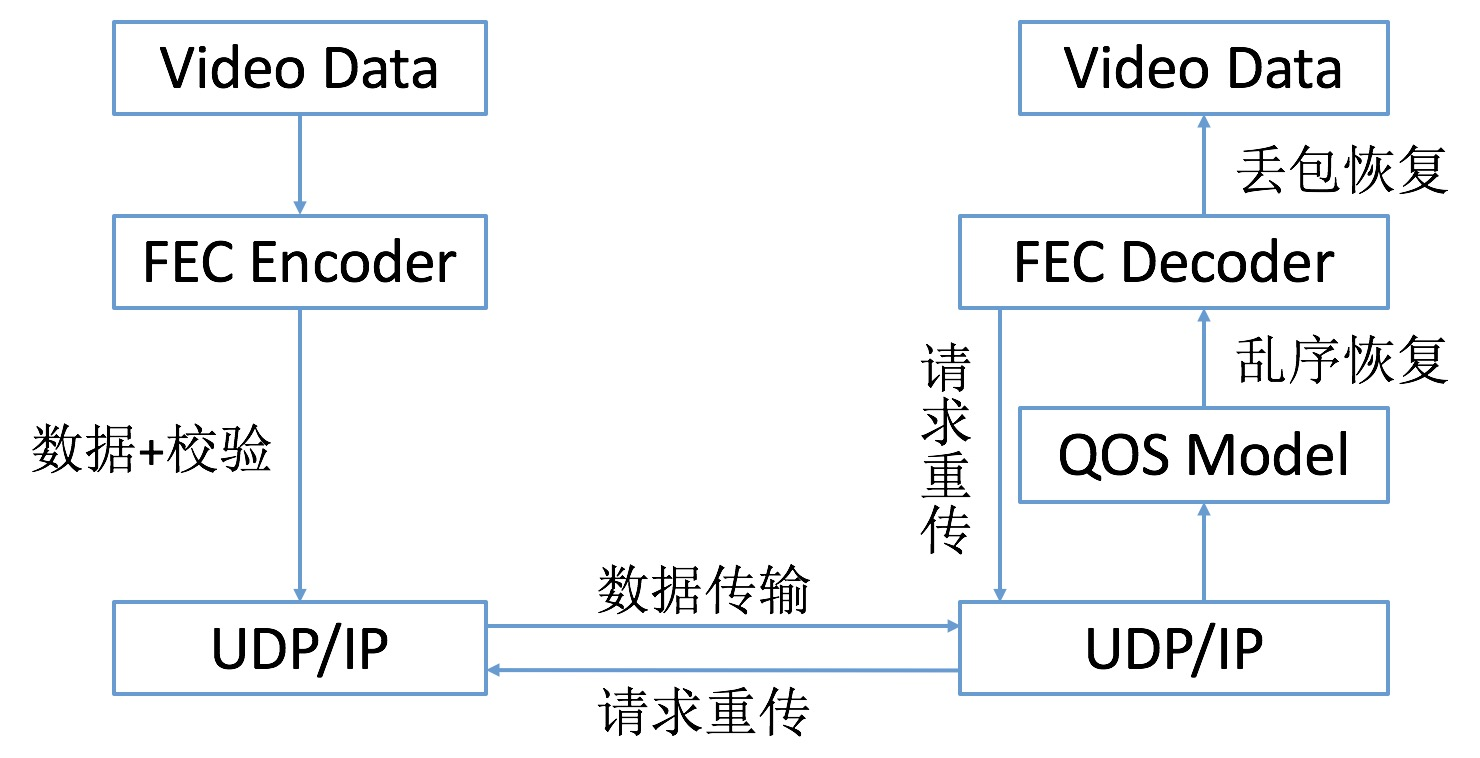
\includegraphics[width=4in]{frame.jpg}
			\caption{算法框架}
			\label{fig:frame}
		\end{figure}
		
		本算法侧重于优化具备随机信道特性的传输链路,即连续丢包的概率远低于单包丢失的情况。
		当丢包率超过前向纠错的恢复上限时,算法无法恢复所有数据,此时若要保证传输的正确性,需要引入请求重传机制。
		
		\subsection{传输协议}
		TCP和UDP是比较常用的传输协议。TCP提供可靠的通信传输,而UDP则常被用于让广播和细节控制交给应用的通信传输。
		\subsubsection{TCP协议}
		TCP是一种面向连接的协议,能提供可靠的传输服务,即TCP通过检验和、序列号、确认应答、重发控制、连接管理以及窗口控制等机制实现可靠性传输。TCP充分实现了数据传输时各种控制功能,可以进行丢包的重发控制,还可以对次序乱掉的分包进行顺序控制。但是这些功能也限制了TCP数据传输的速度,而且使得系统资源要求较高。
		\subsubsection{UDP协议}
		
		UDP是一个非连接的协议,传输数据之前源端和终端不建立连接,当它想传送时就简单地去抓取来自应用程序的数据,并尽可能快地把它扔到网络上。在发送端,UDP传送数据的速度仅仅是受应用程序生成数据的速度、计算机的能力和传输带宽的限制;在接收端,UDP把每个消息段放在队列中,应用程序每次从队列中读一个消息段。由于传输数据不建立连接,因此也就不需要维护连接状态,包括收发状态等,因此一台服务机可同时向多个客户机传输相同的消息。UDP信息包的标题很短,只有8个字节,相对于TCP的20个字节信息包的额外开销很小。UDP使用尽最大努力交付,即不保证可靠交付,因此主机不需要维持复杂的链接状态表(这里面有许多参数)。UDP是面向报文的。发送方的UDP对应用程序交下来的报文,在添加首部后就向下交付给IP层。既不拆分,也不合并,而是保留这些报文的边界,因此,应用程序需要选择合适的报文大小。
		
		基于上述分析,TCP和UDP分别有如下几个特点:
		\begin{itemize}
			\item TCP面向连接;UDP面向无连接
			\item TCP面向字节流;UDP面向报文
			\item TCP首部开销大,有20字节,且占用资源较多;UDP首部开销小,只有8字节,且占用资源少
			\item TCP提供可靠的服务,即,通过TCP连接传送的数据,无差错,不丢失,不重复,且按序到达;UDP尽最大努力交付,即不保证可靠交付;
			\item UDP发送数据速度更快
		\end{itemize}
		
		\subsection{丢包恢复}
		\begin{figure}[h]
			\centering
			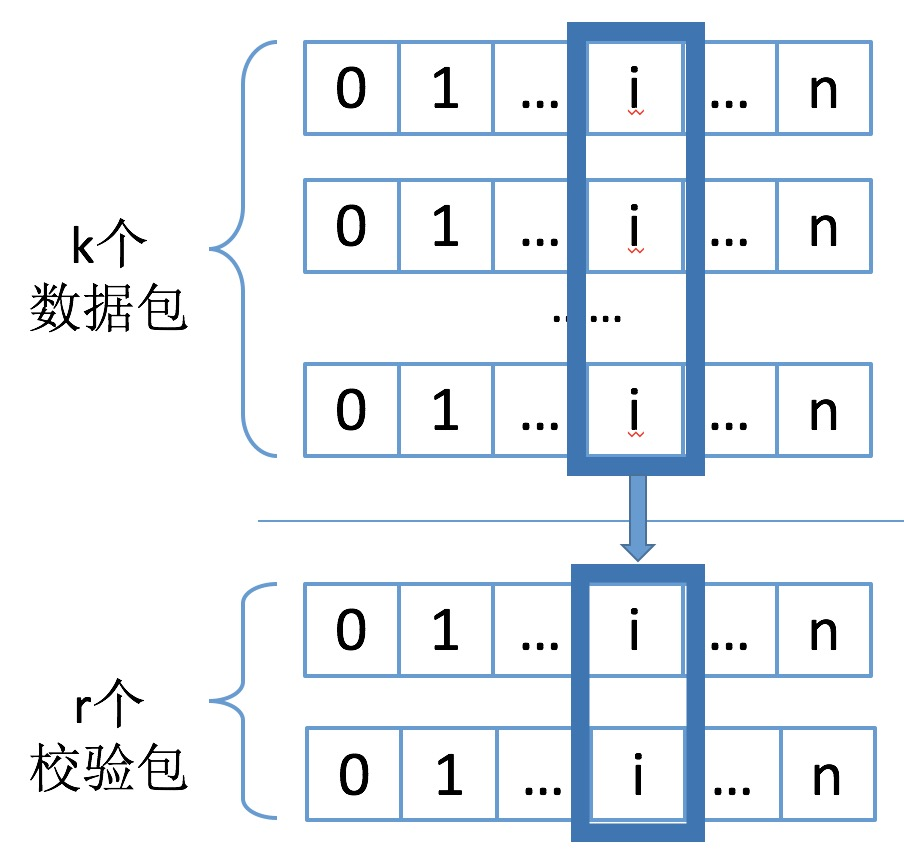
\includegraphics[width=2in]{FEC.jpg}
			\caption{前向纠错算法}
			\label{fig:FEC}
		\end{figure}
		
		前向纠错(FEC)技术近年来广泛应用于信息处理的各个领域。
		FEC算法通过主动提高冗余度来降低丢包重传的频率,从而降低传输延时。
		
		本次实验中的FEC算法在应用层实现,以数据包为单位进行丟包检测与丟包恢复。
		UDP协议保障了包内数据的正确性,我们无需考虑包内纠错,只处理包丢失的情况。
		每k个数据包可以生成r个冗余包,共同构成一个组(Group),即为一个独立的处理单元。
		组内每个包拥有连续的编号,通过读取编号可以判断数据包的丟失情况,并予以恢复
		(冗余包丢失无需恢复)。 
		
		由于冗余性的存在,一个组中任意k个包可以用来重建原始的k个数据包。
		如果丟失数据包数小于或等于r,即可以通过组号信息确定丟失包的相对位置并进行FEC解码,恢复k个原始媒体包。
		这里我们定义冗余包数r与原始媒体包数k的比值为FEC编码冗余度,冗余度越高,抗丟包能力越强,同时传输效率也越低。
		实际应用中,需要找到传输效率与抗丟包能力二者的折中,选择合适的冗余度配置。
		
		实验中采用Vandermonde矩阵RS算法,下面对算法进行简述:
		
		(1)数据包分割
		
		对数据包进行FEC编码运算首先进行的是包内分割,将数据包分割为多个定长单元(字),实验中取字长=8bit。如图\ref{fig:FEC},FEC编码对k个原始媒体包逐字进行处理,生成m个冗余数据包中与之对应的字,包长不足的用0补齐。
		
		(2) 编解码
		
		设k个原始数据包为$D= (D_1,D_2,\dots,D_k)$,r个冗余包为$C=(C_1,C_2,\dots,C_r)$,那么传输组可以表示为$Y= (D,C)$。
		B 为(k+r)xk维FEC生成矩阵,则冗余包生成满足:
		
		$$Y=BD=\left[ \begin{array}{c}I\\G\end{array} \right ]D$$
		
		在接收端,如果接收者收到了Group中的任意k个数据包,即可根据所收到的数据包在组中的位置,从FEC生成矩阵B中提取对应的行, 组成一个新的kxk维矩阵$B'$,显然
		
		$$Y'=B'D$$
		
		如果B’为非奇异矩阵,那么就可以通过如下逆变换得到原始数据包,完成恢复。
		
		$$D=(B')^{-1}Y'$$
		
		设计RS码的关键在于构造系数矩阵G。本实验中我们使用Vandermonde矩阵构建,如下所示:
		
		$$G=
		\left[ \begin{array}{ccccc}
		1      & 1      & 1      & \cdots & 1       \\
		1      & 2      & 2^2    & \cdots & 2^{k-1} \\
		\vdots & \vdots & \vdots & \ddots & \vdots  \\
		1      & r      & r^2    & \cdots & r^{k-1}
		\end{array} 
		\right ]$$
		
		编解码算法中的所有元素运算都在有限域$GF(2^8)$中进行,其中加法采用位异或,乘除法通过查表计算。
		
		\subsection{乱序恢复}
		QOS模块用来处理UDP传输中的包乱序、 包重复、包延时等问题。
		
		客户端发送的每个数据包拥有递增的包序号。
		实验中使用环形队列对接收的数据包进行局部缓存并排序,同时去除接收的重复包以及超时包,最大限度保证接收质量。
		处理后的数据包按包序号从小到大输出给后面的FEC解码环节,后者进行丢包的恢复。
		
		新到数据包根据其序号和队列中已有序号进行对比,计算出其存放位置,若超出队列大小,则直接丢弃。
		设为新到包位置为$P_{new}$,$P_{out}$为即将输出的第一个数据包位置,$N_{new} $为新到包的包序号, $N_{out} $为即将输出的第一个数据包包序号,$Q_{size}$为整个环形队列大小,则:
		$$P_{new} = (P_{out} + (N_{new} - N_{out}))\%Q_{size}$$
		
		找到位置后,首先判断该位置是否已经存在数据包,如果存在,则说明当前包是重复包,直接丢弃;若不存在,则存入队列。
		
		我们用一个线程处理队列的输出,当队列中得到足以恢复一个Group的数据后,将其输出到FEC进行解码,否则保持等待。
		如果等待超过特定的丢包时延t之后,还没有得到足够的数据,就判定为数据丢失,发送丢失信号。
		
		丢包时延是算法中的一个重要参数,如果设置得过小,会发出不必要的丢失信号,系统抵御乱序的能力会变弱;如果设置得过大,则丢包重传的延时变大。
		
		\subsection{请求重传}
		本实验中的请求重传方案只对FEC确定无法恢复的数据包请求,能够尽量的降低重传发起概率,降低延时。
		
		当收到队列的丢失信号后,服务器将队列中第一个缺失数据的编号发送给客户端,由客户端的特定线程接受重传请求,并将编号存入一个队列。
		
		对于情况A,QOS将直接不予等待,将后续接收的包直接交与FEC。对于情况B,QOS将进入“丢包等待时间”,以期收到乱序的包。对于情况C,QOS将发起NACK重传并进入等待,这个等待时间即是“丢包等待时间”又是“重传等待时间”,在等待期内不管是该乱序包到达或者重传包到达,都能满足FEC的恢复条件。
		
\section{项目实现}
		我们使用eclipse进行android开发,使用java的socket编程实现udp协议的数据传输。
		\begin{figure}[h]
			\centering
			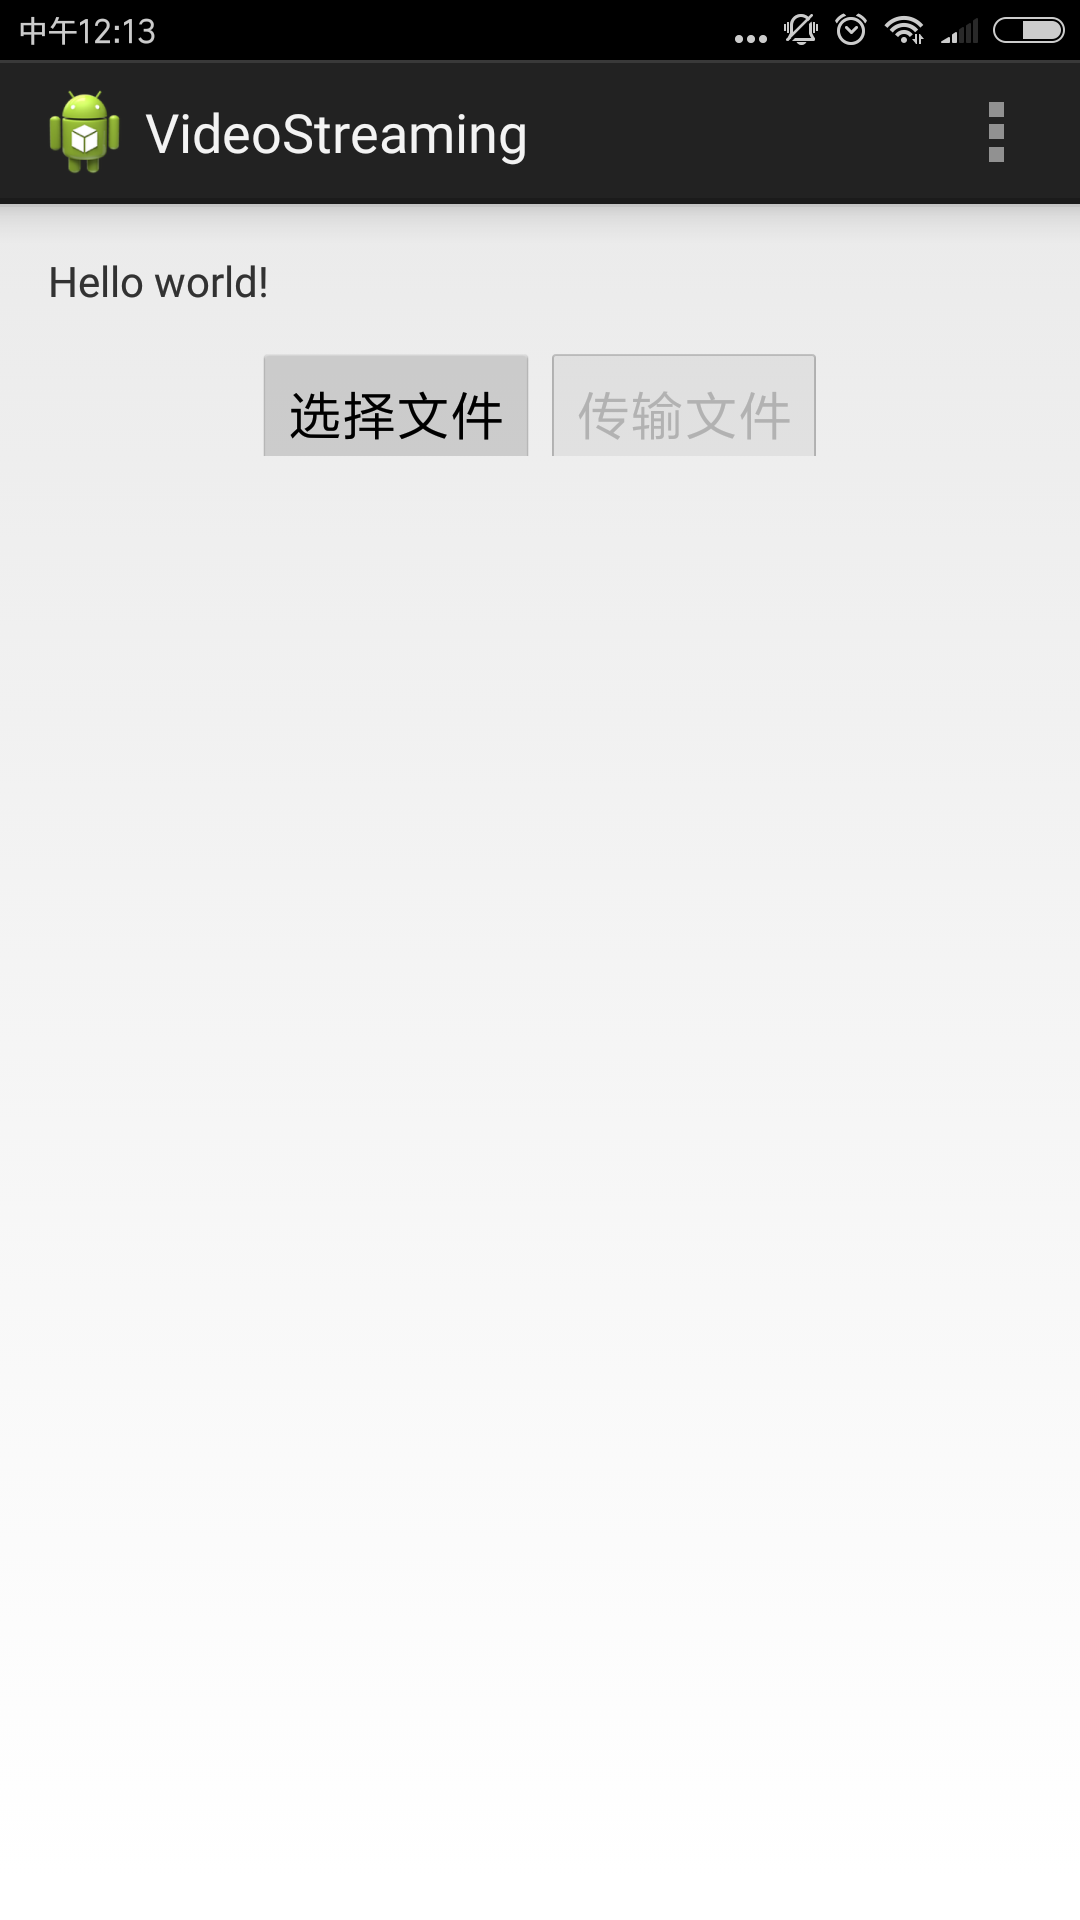
\includegraphics[width=2in]{select.png}
			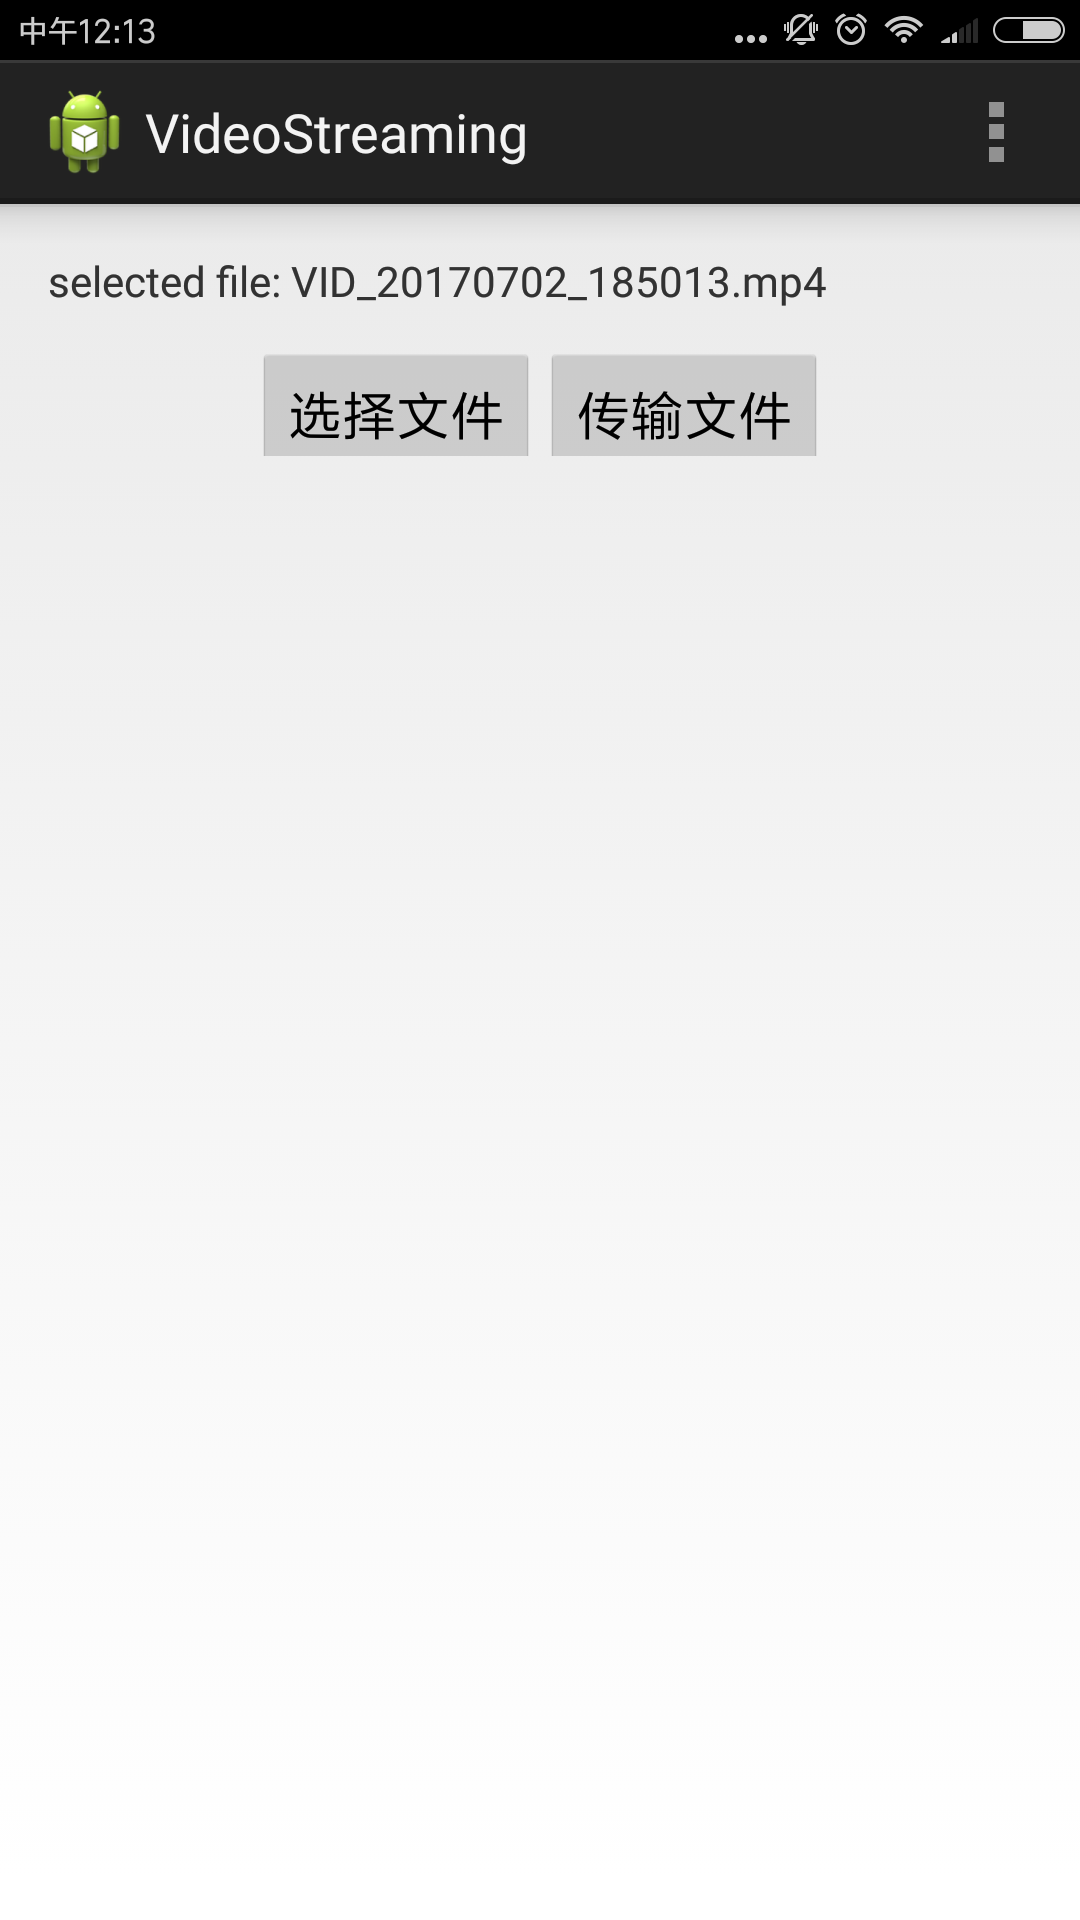
\includegraphics[width=2in]{send.png}
			\caption{android端程序界面}
			\label{fig:android}
		\end{figure}
		
		\subsection{实验环境}
		\begin{itemize}
			\item android. 客户端在android手机上实现了一个应用程序。该程序具有选择文件和传输文件的功能,界面图如图~\ref{fig:android}所示,点击“选择文件”按钮选择想要上传的文件,选择文件后,点击“传输文件”,即开始进行文件上传。\textbf{android测试环境是小米5手机,android 7.0;该应用程序要求android版本最小是andorid 6.0}。
			
			
			在点击“选择文件”按钮时,我们使用android自带的文件选择器进行文件的选择,这时会出现一个文件选择的目录,选择一个短视频,确定即回到主界面;之后我们要获得被选择文件的路径以便后续使用。在文件选择时,android6.0和以前不一样的地方在于,请求文件之前要再次申请权限,仅仅在AndroidManifest.xml文件中申请是不行的。当有文件被选择时,“传输文件”按钮被激活,点击该按钮,主程序会开启一个线程用来传输文件。该线程首先传输一个编号为0的数据包,该数据包的功能是向服务器端传输文件的信息,包括文件大小和文件名。该数据包的前两个字节表示该包的编号(一般设为0),之后四个字节表示文件大小,其他字节表示文件名。客户端发送该数据包之后会等待服务器端的特定信号(成功信号),收到该成功信号之后,客户端会继续传输文件内容;文件内容的包的前两个字节表示的是编号,该编号从1开始,递增至最大(两个字节是足够表示的)。传输文件结束,客户端会发送退出(exit)信号,在收到服务器端的成功回复后(此时服务器端也退出),客户端退出。在传输文件内容过程中,服务器端发现有丢包时,会向客户端发送重传请求,客户端收到重传请求后会暂停目前数据的传输,先重传缺失的包。
			
			\item 服务器端。服务器端的实现是一个eclipse java程序。测试环境是windows 10 64位。在进行文件传输之前,需要先运行服务器端代码,服务器端即进行特定端口的监听,等待数据包的到来。 
		\end{itemize}
		\subsection{默认参数设置}
		默认参数定义在UDPUtils.java中,包括:
		
		包大小:50KB
		
		包编号:从1开始递增
		
		FEC分组:10个数据包+2个校验包
		
		QOS环形队列大小:64
		
\section{实验结果与分析}
		我们采用比对文件MD5值的方式确认文件传输的正确性。
		\subsection{传输速度与冗余}
		由于使用了前向纠错,算法的冗余度基本相当于前向纠错中校验包的比例。
		
		
		\subsection{丢包修复能力}
		在视频传输中,以固定比例随机丢包,测得算法的丢包比例和修复率之间的关系。
		
		
	\end{CJK*}
	
\end{document}
